\chapter{Струны, гравитация, компактификация и T-дуальность}

\lectureoverview{Точечная частица может согласованно двигаться практически в любой гладкой геометрии, но квантовая струна — нет. Её бесконечно многие нулевые колебания зондируют пространство-мишень на всё более коротких масштабах, и эффективная геометрия меняется по мере того, как эти колебания восстанавливаются. Требование, чтобы у этого процесса была неподвижная точка, приводит к \(R_{\mu\nu}=0\), вакуумному уравнению Эйнштейна. Затем мы переходим от этого условия согласованности к компактификации. Окружность даёт как импульсные состояния Калуцы--Клейна, так и состояния намотки струны; их обмен отождествляет окружность радиуса \(R\) с окружностью радиуса \(\alpha'/R\).}

\section{Согласованность как принцип отбора}

Нужно ответить на два вопроса. Почему в теории струн возникает гравитация и почему теория струн гораздо менее снисходительна, чем механика точечной частицы? На самом деле это один и тот же вопрос. Фоновая геометрия допустима только тогда, когда струна может распространяться на ней без того, чтобы сохранялась произвольная зависимость от того, насколько мелко мы разрешаем струну.

Начнём с контрольной задачи: точечная частица, ограниченная гладкой искривлённой поверхностью. Классически она движется по геодезической, внутреннему аналогу прямой линии. Можно аппроксимировать движение многими короткими отрезками, записать разностное уравнение, а затем устремить длину отрезка к нулю. Результатом является обыкновенное дифференциальное уравнение с хорошо определённым непрерывным пределом.

Квантовая механика меняет сумму по историям, но не вывод. Вместо выбора одной классической траектории мы суммируем амплитуды по траекториям на поверхности. Время снова можно разбить на малые шаги, и предел эквивалентно описывается уравнением Schr\"odinger на искривлённом конфигурационном пространстве. Для гладкой поверхности предел сходится к определённым пропагатору и спектру.

\begin{figure}[H]
  \centering
  \includegraphics[width=0.72\textwidth]{lecture_09_figure_01.png}
  \caption{Гладкая траектория на поверхности и ломаная траектория из квантовой суммы, разрезанной по времени. Обе остаются внутренними по отношению к поверхности-мишени.}
  \lectureframe{00:05:10}
  \label{fig:l09-particle-paths}
\end{figure}

\begin{classroomqa}
\audiencequestion{В интеграле по траекториям должны ли все траектории оставаться внутри поверхности? \lecturetimestamp{00:05:39}}
\lecturerresponse{Да. Эта поверхность — конфигурационное пространство частицы, а не лист, вложенный в большее пространство, в котором частица могла бы срезать путь. Каждая промежуточная точка принадлежит поверхности, и все длины и действия вычисляются по её внутренней метрике.}
\end{classroomqa}

Соответствующий вопрос для струны сложнее. Струна задаётся не только положением центра масс. Она несёт бесконечную башню осцилляторов, так что повышение разрешения означает включение большего числа динамических степеней свободы. Теория согласована только тогда, когда наблюдаемые стремятся к пределу по мере восстановления этой башни.

\section{Точечная частица на сфере}

Сфера — простейшая искривлённая тестовая геометрия. Пусть её радиус равен \(R\), и сначала поместим на неё частицу массы \(m\). Для движения вдоль большого круга,
\begin{equation}
  E=\frac{1}{2}mv^2=\frac{p^2}{2m},
  \qquad
  L=pR.
  \label{eq:l09-particle-energy}
\end{equation}
Следовательно,
\begin{equation}
  E=\frac{L^2}{2mR^2}
   =\frac{L^2}{2I},
  \qquad
  I=mR^2.
  \label{eq:l09-rotor-energy}
\end{equation}
Радиус входит через момент инерции. Квантование углового момента даёт привычный спектр жёсткого ротатора, и ничто не зависит от ультрафиолетового обрезания.

\begin{figure}[H]
  \centering
  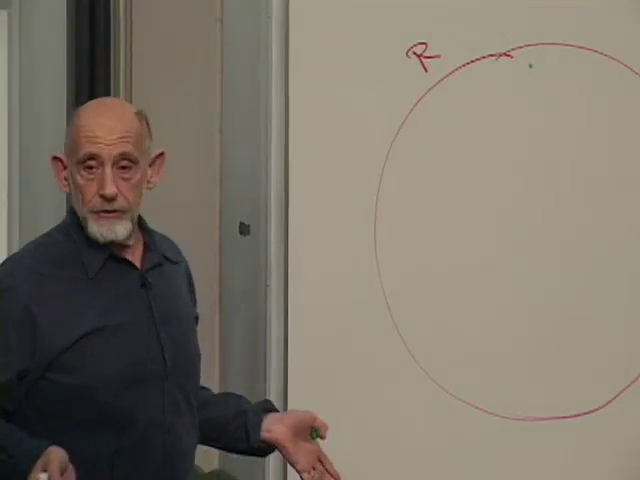
\includegraphics[width=0.74\textwidth]{lecture_09_figure_02.png}
  \caption{Контрольный расчёт для точечной частицы:
  \(p^2/(2m)=L^2/(2mR^2)=L^2/(2I)\).}
  \lectureframe{00:11:25}
  \label{fig:l09-sphere-rotor}
\end{figure}

Этот беспроблемный пример важен. Сама по себе кривизна не является проблемой. Проблема появляется, когда кривизна связана с внутренней квантовой протяжённостью струны.

\section{Вакуумная струна не точечна}

Рассмотрим одну поперечную координату открытой струны и вычтем координату её центра масс. Используемое здесь осцилляторное разложение схематично:
\begin{equation}
  X(\sigma)-X_{\mathrm{cm}}
  \sim
  \sum_{n=1}^{\infty}
  \frac{a_n+a_n^\dagger}{\sqrt n}\cos(n\sigma).
  \label{eq:l09-mode-expansion}
\end{equation}
Существенны косинусные моды, операторы осцилляторов и множитель \(1/\sqrt n\). Точные нормировки не играют роли в рассуждении о размере.
\editorialnote{Точное разложение содержит зависящие от соглашений множители \(\alpha'\), числовые константы и выбор обозначений осцилляторов. В уравнении \eqref{eq:l09-mode-expansion} сохранена только та зависимость, которая нужна для ультрафиолетовой оценки, как и в выводе на доске.}

\begin{figure}[H]
  \centering
  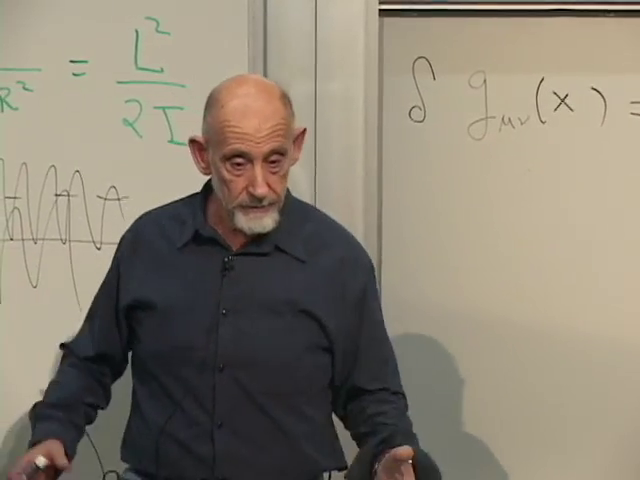
\includegraphics[width=0.78\textwidth]{lecture_09_figure_03.png}
  \caption{Структурное осцилляторное разложение и двойная сумма, получающаяся при его возведении в квадрат.}
  \lectureframe{00:15:20}
  \label{fig:l09-string-modes}
\end{figure}

В осцилляторном вакууме квадрат расстояния от центра масс равен
\begin{align}
  \expect{\bigl(X(\sigma)-X_{\mathrm{cm}}\bigr)^2}_0
  &\sim
  \sum_{n,m\geq1}
  \frac{\cos(n\sigma)\cos(m\sigma)}{\sqrt{nm}}\notag\\
  &\qquad\times
  \bra{0}(a_n+a_n^\dagger)\notag\\
  &\hspace{6em}\times(a_m+a_m^\dagger)\ket{0}.
  \label{eq:l09-size-double-sum}
\end{align}
Большинство членов обращается в нуль. Два оператора уничтожения уничтожают кет-вектор; два оператора рождения оставляют состояние, ортогональное бра-вектору; оператор рождения, за которым следует оператор уничтожения, тоже даёт нулевое вакуумное среднее при таком порядке. Остающаяся свёртка имеет вид
\begin{equation}
  \bra{0}a_n a_m^\dagger\ket{0}=\delta_{nm}.
  \label{eq:l09-vacuum-contraction}
\end{equation}

\begin{figure}[H]
  \centering
  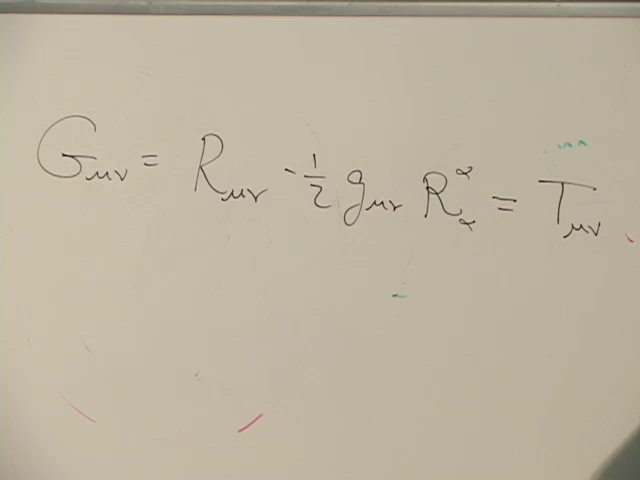
\includegraphics[width=0.74\textwidth]{lecture_09_figure_04.png}
  \caption{Остающаяся вакуумная свёртка сводит двойную сумму по осцилляторам к одной сумме.}
  \lectureframe{00:20:10}
  \label{fig:l09-vacuum-contraction}
\end{figure}

Таким образом
\begin{equation}
  \expect{\bigl(X(\sigma)-X_{\mathrm{cm}}\bigr)^2}_0
  \sim
  \sum_{n=1}^{\infty}\frac{\cos^2(n\sigma)}{n}.
  \label{eq:l09-size-single-sum}
\end{equation}
В произвольной точке вдоль струны, или после усреднения по \(\sigma\), \(\cos^2(n\sigma)\) даёт вклад примерно \(1/2\). При обрезании по модам \(N\),
\begin{equation}
  \expect{\bigl(X-X_{\mathrm{cm}}\bigr)^2}_{0,N}
  \sim
  \frac{1}{2}\sum_{n=1}^{N}\frac{1}{n}
  =\frac{1}{2}\log N+O(1).
  \label{eq:l09-logarithmic-size}
\end{equation}

\begin{figure}[H]
  \centering
  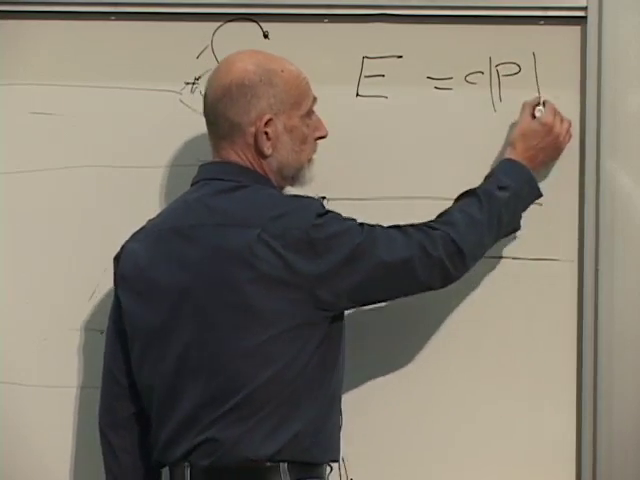
\includegraphics[width=0.72\textwidth]{lecture_09_figure_05.png}
  \caption{На доске получается гармоническая сумма, определяющая разброс основного состояния.}
  \lectureframe{00:22:05}
  \label{fig:l09-harmonic-size}
\end{figure}

Если оставить только, скажем, первые 25 мод, получится конечный размытый объект, но это ещё не струна в непрерывном пределе. При снятии обрезания среднеквадратичный разброс растёт логарифмически. Этот вывод не следует ошибочно понимать как доказательство того, что теория струн в плоском пространстве несогласована. В плоском пространстве движение центра масс и осцилляторные движения разделяются, и тонкие взаимные компенсации в физических амплитудах сохраняют ожидаемую локальность. Растущий размер — это предупреждение. Кривизна показывает, превращается ли оно в провал.

\section{Когда внутреннее размазывание меняет геометрию}

Поместим струну вблизи северного полюса сферы. Когда все осцилляторы выключены, она ведёт себя как только что рассмотренная точечная частица. По мере учёта более высоких мод струна превращается во флуктуирующий клубок, размазанный по шапочке. Её центр по-прежнему может двигаться по сфере, но объект, момент инерции которого входит в энергию вращения, теперь протяжён.

Для оси, проходящей через центр сферы и полюса,
\begin{equation}
  I=\int r_\perp^2\,dm,
  \label{eq:l09-extended-inertia}
\end{equation}
где \(r_\perp\) — перпендикулярное расстояние от элемента струны до этой оси. Точка на экваторе орбиты имеет наибольшее соответствующее плечо. Участки струны, провисающие к оси, дают меньший вклад. При фиксированной полной массе это уменьшает эффективный момент инерции:
\begin{equation}
  I_{\mathrm{eff}}<mR^2.
  \label{eq:l09-inertia-reduction}
\end{equation}
Поэтому энергия вращения выглядит как у точечного объекта на сфере меньшего радиуса,
\begin{equation}
  E_{\mathrm{rot}}
  =\frac{L^2}{2I_{\mathrm{eff}}}
  \equiv \frac{L^2}{2mR_{\mathrm{eff}}^2},
  \qquad R_{\mathrm{eff}}<R.
  \label{eq:l09-effective-radius}
\end{equation}

\begin{classroomqa}
\audiencequestion{Почему момент инерции должен стремиться к нулю, если струна размазывается по большей области? \lecturetimestamp{00:33:23}}
\lecturerresponse{Речь идёт об эффективном описании при последовательном огрублении, а не об утверждении, будто исходное протяжённое распределение сразу имеет нулевой момент инерции. Первая полоса мод превращает точку в размытый сгусток, который движется так, как будто живёт на сфере меньшего радиуса. Следующая полоса разрешает структуру внутри каждого такого сгустка и повторяет ту же ренормализацию. При повторении этого сравнения эффективный радиус сдвигается внутрь.}
\end{classroomqa}

\begin{figure}[H]
  \centering
  \includegraphics[width=0.72\textwidth]{lecture_09_figure_06.png}
  \medskip

  \begin{adjustbox}{max width=\linewidth}
  \begin{tikzpicture}[x=1cm,y=1cm,>=Latex]
    \draw[thick] (0,0) circle (2.15);
    \draw[dashed] (0,-2.55) -- (0,2.55);
    \draw[blue!65!black,thick]
      (-0.22,2.05)
      .. controls (-1.22,1.75) and (-1.52,1.08) .. (-1.06,0.44)
      .. controls (-0.55,-0.10) and (0.35,0.02) .. (1.10,0.68)
      .. controls (1.48,1.12) and (1.16,1.80) .. (0.20,2.05);
    \draw[red!70!black,dashed] (0,0) circle (1.25);
    \draw[->] (2.70,1.55) -- (4.05,1.55);
    \node[align=center] at (3.37,1.98) {add shorter\\modes};
    \draw[thick] (6.15,0) circle (1.25);
    \draw[dashed] (6.15,-1.65) -- (6.15,1.65);
    \draw[blue!65!black,thick]
      (6.00,1.18)
      .. controls (5.42,0.88) and (5.46,0.25) .. (6.02,-0.06)
      .. controls (6.46,-0.28) and (6.90,0.45) .. (6.28,1.18);
    \node at (0,-3.00) {sphere of radius \(R\)};
    \node at (6.15,-2.05) {effective radius \(R_{\mathrm{eff}}\)};
  \end{tikzpicture}
  \end{adjustbox}
  \caption{Струна у северного полюса на доске и аккуратная реконструкция аргумента об эффективном радиусе. Внутренняя пунктирная окружность — это эффективная геометрия, а не вторая физическая оболочка внутри сферы.}
  \lectureframe{00:35:15}
  \label{fig:l09-shrinking-sphere}
\end{figure}

Это утверждение ренормгруппового характера. Конечное обрезание делает струну сгустком с конечным внутренним разрешением. Повышение обрезания меняет механику этого сгустка. На сфере положительной кривизны каждая добавленная оболочка мод делает фон, восстанавливаемый по крупномасштабному движению, меньшим. Если результат никогда не стабилизируется, то на таком фоне не существует струнной теории, независимой от обрезания.

\section{Метрика должна достичь неподвижной точки}

Теперь заменим сферу общей метрикой пространства-мишени \(g_{\mu\nu}(x)\). Добавление тонкой логарифмической оболочки осцилляторных мод изменяет эту метрику на величину, задаваемую локальным симметричным тензором второго ранга. Это изменение должно обращаться в нуль в плоском пространстве и начинаться с двух производных метрики. В ведущем порядке ковариантность оставляет тензор Риччи в качестве подходящего кандидата:
\begin{equation}
  \frac{\partial g_{\mu\nu}}{\partial\log\Lambda}
  =-C\,R_{\mu\nu}+\cdots ,
  \qquad C>0
  \label{eq:l09-ricci-flow}
\end{equation}
в том направлении огрубления, которое использовалось в геометрическом аргументе.
Тогда положительная кривизна сдвигает сферу внутрь, как и требуется.
\editorialnote{Нормировка и знак зависят от того, растёт ли параметр ренормализации в сторону ультрафиолета или инфракрасной области. В стандартных обозначениях мирового листа ведущая бета-функция метрики имеет вид \(\beta^g_{\mu\nu}=\alpha'R_{\mu\nu}+\cdots\). Инвариантное утверждение, используемое здесь, состоит в том, что независимость от обрезания требует обращения в нуль бета-функции и, следовательно, \(R_{\mu\nu}\) в этом порядке.}

\begin{figure}[H]
  \centering
  \includegraphics[width=0.76\textwidth]{lecture_09_figure_07.png}
  \caption{Изменение метрики схематически записано как минус тензор Риччи, а рядом с ним нарисована кривая сглаживания.}
  \lectureframe{00:43:00}
  \label{fig:l09-ricci-flow-board}
\end{figure}

\begin{classroomqa}
\audiencequestion{Где в этом уравнении потока появляется отсечка по осцилляторным модам \(N\)? \lecturetimestamp{00:43:38}}
\lecturerresponse{Это и есть переменная масштаба. Сумма, определяющая размер струны, меняется логарифмически при изменении наивысшей включённой моды, так что естественным параметром эволюции служит \(\log N\), или, эквивалентно, \(\log\Lambda\). Уравнение \eqref{eq:l09-ricci-flow} описывает бесконечно малое изменение, вызываемое одной логарифмической оболочкой мод.}
\end{classroomqa}

Допустимый фон является неподвижной точкой этого потока. В ведущем порядке,
\begin{equation}
  \boxed{R_{\mu\nu}=0.}
  \label{eq:l09-ricci-flat}
\end{equation}
Равенство нулю тензора Риччи не означает, что обращается в нуль каждая компонента тензора Римана. Гравитационные волны, например, могут иметь ненулевую кривизну в вакууме, удовлетворяя при этом \(R_{\mu\nu}=0\).

\subsection{То же условие есть вакуумное уравнение Эйнштейна}

При опущенных стандартных константах уравнение Эйнштейна имеет вид
\begin{equation}
  G_{\mu\nu}
  \equiv
  R_{\mu\nu}-\frac12 g_{\mu\nu}R
  =T_{\mu\nu}.
  \label{eq:l09-einstein}
\end{equation}

\begin{figure}[H]
  \centering
  \includegraphics[width=0.78\textwidth]{lecture_09_figure_08.png}
  \caption{Тензор Эйнштейна и тензор энергии-импульса на доске.}
  \lectureframe{00:47:15}
  \label{fig:l09-einstein-board}
\end{figure}

В вакууме \(T_{\mu\nu}=0\). Взятие следа в \(D\) измерениях пространства-времени даёт
\begin{equation}
  0=g^{\mu\nu}G_{\mu\nu}
   =\left(1-\frac{D}{2}\right)R.
  \label{eq:l09-einstein-trace}
\end{equation}
При \(D\neq2\) имеем \(R=0\), и подстановка этого обратно в \eqref{eq:l09-einstein} даёт \(R_{\mu\nu}=0\). Тем самым условие, что струна утрачивает зависимость от отсечки, и есть вакуумное уравнение гравитационного поля. Гравитация не была добавлена к теории; она возникла как цена согласованности.

Слово \emph{вакуум} не означает, что ничего не происходит. Оно означает, что в данной области нет источника энергии-импульса. Уравнения Максвелла без источников допускают электромагнитные волны, а уравнения Эйнштейна без источников — гравитационные волны. Геометрия может быть динамической, даже когда её тензор Риччи обращается в нуль.

\begin{classroomqa}
\audiencequestion{Связано ли это условие с конформной инвариантностью?
\lecturetimestamp{00:52:20}}
\lecturerresponse{Да, хотя на записи вопрос частично неразборчив. Здесь существенна конформная инвариантность квантовой теории на \emph{листе мира}. Именно требование, чтобы масштабная аномалия листа мира обращалась в нуль, заставляет бета-функцию метрики обращаться в нуль. Это не следует путать с требованием конформной инвариантности самого пространства-времени.}
\end{classroomqa}

Есть и второе условие согласованности. Конформная инвариантность на листе мира также фиксирует критическую размерность пространства-времени: десять для суперструн и двадцать шесть для бозонной струны. Поэтому одного лишь обращения в нуль тензора Риччи недостаточно: это не полный список требований, но именно эта часть наиболее прямо выявляет уравнение Эйнштейна.

\section{Компактные измерения, а не отсутствующие измерения}

Фон суперструнной теории имеет девять пространственных измерений и одно временное измерение. Наш макроскопический мир проявляет лишь три протяжённых пространственных направления, так что шесть пространственных измерений должны быть скрыты или иным образом сделаны недоступными на обычных масштабах. Компактификация сохраняет их как подлинные направления, но придаёт им малый конечный размер.

\begin{classroomqa}
\audiencequestion{Если у разных наблюдателей разные часы, означает ли это, что имеется более одного временного измерения? \lecturetimestamp{00:56:59}}
\lecturerresponse{Нет. Множество часов — это множество приборов, измеряющих координаты в одном пространстве-времени; они не создают независимых времениподобных направлений. Дополнительные измерения, рассматриваемые здесь, являются пространственными. Привычные квантовые и причинные конструкции не дают сопоставимой согласованной теории с несколькими локальными временными направлениями, так что эта возможность не входит в данную модель компактификации.}
\end{classroomqa}

Представьте существ, которые считают, что их мир — это линия. При низком разрешении они могут двигаться только вперёд и назад. Однако под достаточно сильным микроскопом выясняется, что эта линия на самом деле является очень тонким цилиндром. Маленькое существо может перемещаться как по его круговому направлению, так и вдоль его длины. Второе направление присутствовало всегда; длина его окружности была слишком мала, чтобы грубые зонды могли её различить.

\begin{figure}[H]
  \centering
  \includegraphics[width=0.78\textwidth]{lecture_09_figure_09.png}
  \caption{Узкий цилиндр и траектории, обвивающие его скрытое круговое направление.}
  \lectureframe{01:01:00}
  \label{fig:l09-hidden-cylinder}
\end{figure}

Цилиндр можно представить как полосу, у которой отождествлены верхний и нижний края. При пересечении верхнего края возвращение происходит через нижний в той же продольной координате. Ни один из этих краёв не является физической границей. Ту же операцию можно выполнить в двух направлениях: отождествить левый и правый края прямоугольника, а также его верхний и нижний края. В результате получается двумерный тор.

\begin{figure}[H]
  \centering
  \includegraphics[width=0.76\textwidth]{lecture_09_figure_10.png}
  \medskip

  \begin{tikzpicture}[x=0.82cm,y=0.82cm,>=Latex]
    \draw[thick] (0,0) rectangle (4,2.15);
    \draw[blue!65!black,->] (0,2.48) -- (4,2.48);
    \draw[blue!65!black,->] (4,-0.34) -- (0,-0.34);
    \node at (2,-0.82) {one periodic direction};
    \draw[thick] (6.1,0) rectangle (10.1,2.15);
    \draw[blue!65!black,->] (6.1,2.48) -- (10.1,2.48);
    \draw[blue!65!black,->] (10.1,-0.34) -- (6.1,-0.34);
    \draw[red!70!black,->] (5.76,0) -- (5.76,2.15);
    \draw[red!70!black,->] (10.44,2.15) -- (10.44,0);
    \node at (8.1,-0.82) {two periodic directions};
  \end{tikzpicture}
  \caption{Изображённая на доске пластина и её аккуратное описание через фундаментальную область.
  Отождествление одной пары краёв даёт цилиндр; отождествление обеих пар даёт
  тор.}
  \lectureframe{01:04:40}
  \label{fig:l09-periodic-identification}
\end{figure}

Тор — это прежде всего топология, а уже потом поверхность в форме бублика в трёхмерном пространстве. Если разрезать тор один раз, получится цилиндр; если разрезать ещё раз, получится прямоугольник, при условии что отождествления краёв не забыты. На этом прямоугольнике можно задать плоскую метрику, так что получающийся плоский тор локально имеет нулевую кривизну Римана и, разумеется, является риччи-плоским.

Прямая траектория на прямоугольнике продолжается по прямой через отождествлённый край. Если её наклон задаётся рациональным отношением двух периодов, траектория в конце концов замыкается. Если это отношение иррационально, она никогда не замыкается и становится всюду плотной на торе.

\begin{figure}[H]
  \centering
  \includegraphics[width=0.76\textwidth]{lecture_09_figure_11.png}
  \caption{Повторяющиеся прямые отрезки в фундаментальной области представляют
  одну непрерывную траекторию на торе.}
  \lectureframe{01:11:00}
  \label{fig:l09-torus-trajectory}
\end{figure}

Торы более высокой размерности строятся таким же образом. Куб, у которого отождествлена каждая пара противоположных граней, представляет собой трёхмерный тор, а шесть компактных направлений можно представить шестимерным тором. Не следует пытаться вложить все эти объекты в обычное трёхмерное пространство; описание через отождествление граней является внутренним и полным.

\begin{classroomqa}
\audiencequestion{Должно ли дополнительное измерение обязательно замыкаться на себя?
\lecturetimestamp{01:15:03}}
\lecturerresponse{Нет, это не следует ни из какой теоремы. Оно могло бы быть некомпактным, но тогда обычно проявлялось бы как ещё одно протяжённое направление в наблюдаемом нами мире на больших расстояниях. Компактность — самый простой способ согласовать дополнительные измерения с их кажущимся отсутствием. Почему природа выбирает ту или иную компактификацию, — отдельный динамический вопрос.}
\end{classroomqa}

\begin{classroomqa}
\audiencequestion{Почему предполагают, что ненаблюдаемые измерения — это обычные пространственные направления, свёрнутые таким образом, а не нечто совершенно иное? \lecturetimestamp{01:15:51}}
\lecturerresponse{Потому что это чётко сформулированная, решаемая гипотеза, а не потому, что доказано, будто это единственно возможное описание природы. Компактные пространственные многообразия позволяют строить согласованные примеры и вычислять их спектры. Более экзотические возможности должны заслужить своё место, сделав то же самое.}
\end{classroomqa}

\begin{classroomqa}
\audiencequestion{Расстояния на привычном торе в форме бублика не похожи на расстояния в прямоугольнике. Какая именно геометрия имеется в виду?
\lecturetimestamp{01:18:11}}
\lecturerresponse{Термин \emph{тор} задаёт отождествления, а не единственную метрику. Тор, вложенный как «бублик», наследует искривлённую метрику трёхмерного пространства. Прямоугольник с периодически отождествлёнными сторонами несёт плоскую метрику. Топология у них одна и та же, а геометрия различна; для простой компактификации мы имеем в виду плоскую.}
\end{classroomqa}

\section{Параметры формы плоского тора}

Даже плоский двумерный тор не единственен. Его фундаментальный параллелограмм характеризуется общей площадью, отношением сторон и сдвигом. Изменение этих параметров меняет расстояния и, следовательно, спектр, не изменяя топологии.

\begin{figure}[H]
  \centering
  \includegraphics[width=0.74\textwidth]{lecture_09_figure_12.png}
  \medskip

  \begin{tikzpicture}[x=0.9cm,y=0.9cm,>=Latex]
    \draw[thick] (0,0) rectangle (3.4,2.1);
    \draw[<->] (0,-0.35) -- node[below] {\(L_1\)} (3.4,-0.35);
    \draw[<->] (-0.35,0) -- node[left] {\(L_2\)} (-0.35,2.1);
    \draw[thick] (5.4,0) -- (8.8,0) -- (9.7,2.1) -- (6.3,2.1) -- cycle;
    \draw[dashed] (5.4,0) -- (6.3,2.1);
    \draw[->] (5.75,2.48) -- node[above] {shear} (6.45,2.48);
    \node at (1.7,-1.00) {area and aspect ratio};
    \node at (7.55,-1.00) {complex structure};
  \end{tikzpicture}
  \caption{Прямоугольная и скошенная фундаментальные области, используемые при обсуждении модулей тора.}
  \lectureframe{01:23:00}
  \label{fig:l09-torus-moduli}
\end{figure}

Для двумерного тора удобно кодировать форму комплексным числом \(\tau=\tau_1+i\tau_2\): действительная часть задаёт сдвиг, а мнимая — отношение сторон после выделения общего масштаба. Перестановка двух базисных циклов или замена их целочисленного базиса может привести к тому, что кажущиеся разными параллелограммы описывают один и тот же тор.

\begin{classroomqa}
\audiencequestion{Что произойдёт, если перед отождествлением перевернуть одну сторону? \lecturetimestamp{01:24:20}}
\lecturerresponse{Это приводит к другой топологии. Отождествление с отражением даёт неориентируемую поверхность — бутылку Клейна, а не обычный тор.}
\end{classroomqa}

\begin{classroomqa}
\audiencequestion{Что, если скручивание вдоль края неравномерно?
\lecturetimestamp{01:25:01}}
\lecturerresponse{Гладкую неравномерную деформацию можно перенести в метрику на фундаментальной области. Топологическое отождествление и геометрические данные нужно различать: изменение склейки может изменить топологию, тогда как гладкое изменение расстояний меняет метрику.}
\end{classroomqa}

\editorialnote{Для плоского двумерного тора площадь является простейшим модулем Кэлера, а \(\tau\) — модулем комплексной структуры. Непрерывная сдвиговая деформация входит в \(\tau\). Де́нов скрут, напротив, является дискретной операцией группы классов отображений, представляемой как \(\tau\mapsto\tau+1\); сам по себе он не является непрерывным модулем. Это уточняет намеренно неформальную терминологию, использованную при обсуждении у доски.}

Плоские торы полезны тем, что сразу удовлетворяют условию согласованности, но их симметрия слишком велика для реалистической модели физики частиц. Более сложные риччи-плоские пространства, в частности многообразия Calabi--Yau, дают более богатые компактификации. Их детальное построение выходит за рамки этого обсуждения; сам принцип остаётся тем же.

\section{Определение компактной окружности по её спектру}

После перерыва сведём компактное пространство к одной окружности длины \(2\pi R\). Волновая функция должна быть однозначной после одного обхода:
\begin{equation}
  e^{ip_c(x+2\pi R)/\hbar}=e^{ip_cx/\hbar}.
\end{equation}
Следовательно,
\begin{equation}
  p_cR=n\hbar,
  \qquad
  p_c=\frac{n\hbar}{R},
  \qquad n\in\mathbb Z.
  \label{eq:l09-kk-momentum}
\end{equation}

\begin{figure}[H]
  \centering
  \includegraphics[width=0.74\textwidth]{lecture_09_figure_13.png}
  \caption{Длина компактной окружности \(2\pi R\) и квантованный импульс
  \(p_c=n\hbar/R\).}
  \lectureframe{01:32:15}
  \label{fig:l09-kk-board}
\end{figure}

Для безмассовой частицы в полном пространстве-времени
\begin{equation}
  E=c|\mathbf P|.
  \label{eq:l09-massless-dispersion}
\end{equation}

\begin{figure}[H]
  \centering
  \includegraphics[width=0.70\textwidth]{lecture_09_figure_14.png}
  \caption{Безмассовое дисперсионное соотношение, используемое для переинтерпретации компактного
  импульса как массы в пространстве меньшей размерности.}
  \lectureframe{01:33:45}
  \label{fig:l09-massless-board}
\end{figure}

Разложим импульс на некомпактную и компактную части и положим
\(c=\hbar=1\):
\begin{equation}
  E^2=\mathbf p_{\mathrm{large}}^2+\frac{n^2}{R^2}.
  \label{eq:l09-kk-dispersion}
\end{equation}
Наблюдатель, который не может различить компактное направление, сравнивает это с
\(E^2=\mathbf p_{\mathrm{large}}^2+m^2\) и заключает, что существует башня масс
\begin{equation}
  m_n=\frac{|n|}{R}.
  \label{eq:l09-kk-masses}
\end{equation}
Два знака \(n\) описывают противоположные компактные импульсы при одной и той же положительной энергии, а не положительные и отрицательные массы. Поэтому шаг \(1/R\) позволяет спектроскопически определить радиус. Это механизм Kaluza--Klein: импульс в скрытом направлении проявляется как масса в видимых измерениях.

\section{Состояния с намоткой дополняют спектр}

У замкнутой струны есть возможность, недоступная точечной частице: она может наматываться на окружность. Если число намотки равно \(w\), струна замыкается лишь после того, как покрывает компактное направление \(w\) раз. Её длина равна \(2\pi |w|R\), поэтому натяжение даёт энергию
\begin{equation}
  m_w
  =2\pi T\,|w|R
  =\frac{|w|R}{\alpha'}.
  \label{eq:l09-winding-mass}
\end{equation}
В лекции выбраны единицы с \(\alpha'=1\), так что это сводится к
\begin{equation}
  m_w=|w|R.
  \label{eq:l09-winding-lecture-units}
\end{equation}
Положительные и отрицательные \(w\) соответствуют противоположным ориентациям обхода окружности.

\begin{figure}[H]
  \centering
  \includegraphics[width=0.76\textwidth]{lecture_09_figure_15.png}
  \caption{Замкнутая струна, намотанная на компактный цилиндр; компактный
  радиус отмечен на доске.}
  \lectureframe{01:39:45}
  \label{fig:l09-winding-board}
\end{figure}

Таким образом, компактная окружность порождает две взаимодополняющие башни:
\begin{equation}
  m_n=\frac{|n|}{R},
  \qquad
  m_w=\frac{|w|R}{\alpha'}.
  \label{eq:l09-two-towers}
\end{equation}
Когда \(R\) велик, уровни импульса расположены тесно, а состояния с намоткой тяжелы. Когда \(R\) мал, уровни импульса расположены редко, а состояния с намоткой легки.

\begin{figure}[H]
  \centering
  \begin{tikzpicture}[x=1cm,y=0.9cm,>=Latex]
    \draw[->] (0,0) -- (0,4.7) node[above] {\(m\)};
    \foreach \y/\lab in {0/0,1.1/{1/R},2.2/{2/R},3.3/{3/R},4.4/{4/R}} {
      \draw (-0.16,\y) -- (0.16,\y);
      \node[left] at (-0.22,\y) {\(\lab\)};
    }
    \node at (0,-0.62) {momentum};
    \draw[<->,very thick,blue!65!black] (2.05,2.15) -- (4.05,2.15)
      node[midway,above] {\(R\leftrightarrow\alpha'/R\)};
    \draw[->] (6.1,0) -- (6.1,4.7) node[above] {\(m\)};
    \foreach \y/\lab in {0/0,1.1/{R/\alpha'},2.2/{2R/\alpha'},3.3/{3R/\alpha'},4.4/{4R/\alpha'}} {
      \draw (5.94,\y) -- (6.26,\y);
      \node[right] at (6.32,\y) {\(\lab\)};
    }
    \node at (6.1,-0.62) {winding};
  \end{tikzpicture}
  \caption{Башни импульса и намотки меняются местами, когда радиус
  обращается в струнных единицах.}
  \label{fig:l09-dual-mass-towers}
\end{figure}

\section{T-дуальность: малые и большие окружности описывают одну и ту же физику}

Эти две башни переставляются преобразованием
\begin{equation}
  R\longleftrightarrow\frac{\alpha'}{R},
  \qquad
  n\longleftrightarrow w.
  \label{eq:l09-t-duality}
\end{equation}
В единицах, использованных на доске, \(\alpha'=1\), так что это просто
\(R\leftrightarrow1/R\). При самодуальном радиусе
\(R=\sqrt{\alpha'}\) масштабы импульса и намотки совпадают.

\begin{figure}[H]
  \centering
  \includegraphics[width=0.74\textwidth]{lecture_09_figure_16.png}
  \caption{Разреженная и плотная лестницы масс, сопоставленные на доске, когда
  радиус проходит через самодуальный масштаб.}
  \lectureframe{01:43:00}
  \label{fig:l09-duality-board}
\end{figure}

Обмен элементарных формул масс — лишь видимая часть результата. Осцилляторные состояния замкнутой струны и амплитуды рассеяния тоже согласованно сопоставляются. Окружность меньше струнного масштаба — это не новая всё более крошечная геометрия; у неё есть эквивалентное описание как у большей дуальной окружности. Точечные частицы не допускают такого отождествления, потому что у них есть моды импульса, но нет мод намотки.

\begin{classroomqa}
\audiencequestion{Это просто то же самое, что поменять местами вертикальное и горизонтальное направления? \lecturetimestamp{01:44:38}}
\lecturerresponse{Нет. Здесь меняются местами два разных квантовых числа: импульс по окружности и число раз, которое замкнутая струна оборачивает окружность. При этом радиус должен одновременно обратиться.}
\end{classroomqa}

\begin{classroomqa}
\audiencequestion{Относятся ли описания при \(R<\sqrt{\alpha'}\) и
\(R>\sqrt{\alpha'}\) только к бозонам или также к фермионам?
\lecturetimestamp{01:46:30}}
\lecturerresponse{Дуальность является симметрией полной компактфицированной теории струн, а не только простой бозонной лестницы масс, использованной для её демонстрации. Подробное сопоставление секторов зависит от теории, но эквивалентность малого--большого радиуса не ограничивается одним видом частиц.}
\end{classroomqa}

\begin{classroomqa}
\audiencequestion{Сравниваемые два состояния — это открытые струны или замкнутые
струны? \lecturetimestamp{01:47:32}}
\lecturerresponse{Это состояния замкнутой струны. Свободно распространяющаяся
замкнутая струна может наматываться на компактную окружность. Обычная открытая струна со свободными
концами не несёт того же сохраняющегося числа намотки.}
\end{classroomqa}
\editorialnote{В более полном рассмотрении открытых струн T-дуальность обменивает
граничные условия Неймана и Дирихле и вводит D-браны. Поэтому
T-дуальность открытых струн богаче, чем простое копирование формулы намотки для замкнутой струны.}

\begin{classroomqa}
\audiencequestion{Аналогична ли эта перестановка обмену пространства и
времени вблизи горизонта чёрной дыры? \lecturetimestamp{01:48:00}}
\lecturerresponse{Нет. Горизонтные координаты и причинный характер — это
другой вопрос. Здесь два описания относятся к одной компактной пространственной
окружности и к обмену её секторов импульса и намотки.}
\end{classroomqa}

\begin{classroomqa}
\audiencequestion{Решает ли это проблему самоэнергии на малых расстояниях,
вводя минимальную длину? \lecturetimestamp{01:48:35}}
\lecturerresponse{Это показывает, что радиусы ниже струнного масштаба не задают
новых неэквивалентных фонов окружности: при уменьшении \(R\) дальше самодуальной
точки дуальный радиус увеличивается. Это точное струнное препятствие для
зондирования сколь угодно малой геометрии окружности, хотя не следует превращать
это в утверждение, будто всякое мыслимое понятие расстояния имеет одну универсальную
жёсткую нижнюю границу.}
\end{classroomqa}

\section{Почему сектора намотки нельзя опустить}

\begin{classroomqa}
\audiencequestion{Могли бы мы определить теорию, используя только струны без намотки,
и исключить состояния с намоткой? \lecturetimestamp{01:48:56}}
\lecturerresponse{Нет. Взаимодействия замкнутых струн порождают их. Растяните
петлю без намотки вдоль компактного направления так, чтобы один её участок шёл
по окружности в одну сторону, а другой — в противоположную. Суммарная
намотка по-прежнему равна нулю. Затем пересоединение может расщепить петлю на две
замкнутые струны с намотками \(+1\) и \(-1\). Пара может разойтись, так что
состояния с намоткой должны входить в спектр, даже если в начальном состоянии их
не было.}
\end{classroomqa}

\begin{figure}[H]
  \centering
  \includegraphics[width=0.74\textwidth]{lecture_09_figure_17.png}
  \caption{Растянутая петля с нулевой намоткой, расположенная вдоль компактного
  направления перед пересоединением.}
  \lectureframe{01:50:30}
  \label{fig:l09-winding-pair-before}
\end{figure}

\begin{figure}[H]
  \centering
  \includegraphics[width=0.72\textwidth]{lecture_09_figure_18.png}
  \medskip

  \begin{tikzpicture}[x=0.9cm,y=0.9cm,>=Latex]
    \draw[thick] (0,0) ellipse (1.0 and 1.55);
    \draw[blue!65!black,thick]
      (0.08,1.35) .. controls (2.0,1.15) and (2.0,-1.15) .. (0.08,-1.35);
    \draw[red!70!black,thick]
      (-0.08,-1.35) .. controls (-2.0,-1.15) and (-2.0,1.15) .. (-0.08,1.35);
    \node at (0,-2.15) {net \(w=0\)};
    \draw[->,thick] (2.45,0) -- (3.75,0) node[midway,above] {split};
    \draw[thick] (5.05,0.62) ellipse (0.68 and 1.02);
    \draw[blue!65!black,very thick,->]
      (5.05,1.64) arc[start angle=90,end angle=-250,x radius=0.68,y radius=1.02];
    \node at (5.05,-0.82) {\(w=+1\)};
    \draw[thick] (7.45,0.62) ellipse (0.68 and 1.02);
    \draw[red!70!black,very thick,<-]
      (7.45,1.64) arc[start angle=90,end angle=-250,x radius=0.68,y radius=1.02];
    \node at (7.45,-0.82) {\(w=-1\)};
  \end{tikzpicture}
  \caption{Показанная на доске разделившаяся намотанная петля и аккуратная реконструкция
  рождения пары намотка--антинамотка. Полная намотка остаётся нулевой.}
  \lectureframe{01:51:30}
  \label{fig:l09-winding-pair-after}
\end{figure}

\begin{classroomqa}
\audiencequestion{Требует ли рождение пары с намоткой дополнительной энергии?
\lecturetimestamp{01:52:11}}
\lecturerresponse{Да. Растяжение струны требует энергии натяжения, а конечные
намотанные струны имеют массы из
\eqref{eq:l09-winding-mass}. Столкновение с достаточно большой энергией может
породить пару, точно так же как столкновение может породить частицу и её
античастицу, сохраняя соответствующий сохраняющийся заряд.}
\end{classroomqa}

\section{Можно ли услышать форму струнного фона?}

В обычной компактфицированной теории частиц шаг спектра
Kaluza--Klein позволяет определить радиус: пытаются услышать форму
компактного пространства по его нормальным модам. Теория струн делает обратную
задачу более тонкой. Импульсные моды слышат \(1/R\), моды намотки слышат
\(R/\alpha'\), и полный спектр не меняется при перестановке одного с другим.
Два радиуса, которые геометрия точечных частиц считает различными,
оказываются одним струнным фоном, описанным в дуальных переменных.

Таким образом, лекция пришла к обоим обещанным выводам одним путём. Ультрафиолетовая согласованность заставляет метрику пространства-мишени удовлетворять уравнению Эйнштейна в вакууме, так что гравитация неизбежна. Затем компактификация превращает скрытую геометрию в спектры частиц, но состояния с намоткой не позволяют этому спектру приписывать единственный классический радиус ниже струнного масштаба. Согласованность не просто отбирает, какие геометрии допустимы; через T-дуальность она меняет и само то, что вообще считается различной геометрией.
